%Example of use of oxmathproblems latex class for problem sheets
\documentclass{oxmathproblems}

%(un)comment this line to enable/disable output of any solutions in the file
%\printanswers

%define the page header/title info
\trinityterm{STU33009}
\course{Statistical Methods for Computer Science}
\assignmentnumber{4}

% add further contact details to footer if desired,
%e.g. email address, or name and email address
\contact{Hamza Mughees, 17329860}

\usepackage{tikz}
\usepackage{pgfplots}
\usepackage{subcaption}

\begin{document}

\begin{questions}

\miquestion
\begin{parts}
    \part The sum of the two dice rolls must be to 2, which can only happen if both roll a 1. Therefore the event is (1,1).
    \part The two dice rolls must add to 3. Therefore the event is \{(1,2),(2,1)\}.
    \part The dice rolls must sum to 4. Therefore the event is \{(1,3),(2,2),(3,1)\}
    \part The total number of possible combinations is $6^2=36$. The given event consists of 3 possible outcomes. Therefore the probability is $\dfrac{3}{36}=\dfrac{1}{12}=0.08333333333$
\end{parts}

\miquestion
\begin{parts}
    \part The possible values of $X$ are \{3,1,-1,3\}
    \part The total number of outcomes possible is $2^3=8$. Therefore,
    $$P(X=-3)=\frac{1}{8}=0.125$$
    \part In order to get $X=-1$, there must be one head within the combination. This head can be the outcome of any one of the three flips,
    $$P(X=-1)={3\choose1}\cdot\frac{1}{8}=\frac{3}{8}=0.375$$
    \part The following are the PMF and the CDF of $X$
    \begin{figure}[h]
    \begin{subfigure}{.5\textwidth}
        \centering
        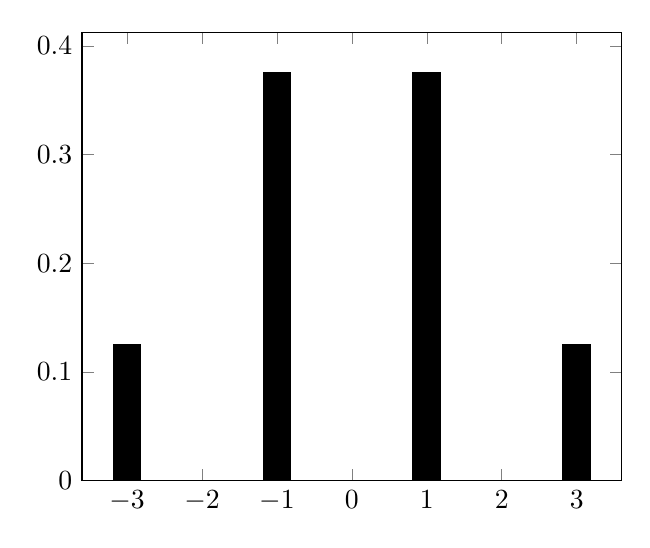
\begin{tikzpicture}
        \begin{axis}[
            ymin=0
        ]
        \addplot[ybar, fill=black] coordinates {
            (-3,0.125)
            (-1,0.375)
            (1,0.375)
            (3,0.125)
        };
        \end{axis}
        \end{tikzpicture}
        \caption{PMF}
        \label{fig:cdf1}
    \end{subfigure}
    \begin{subfigure}{.5\textwidth}
        \centering
        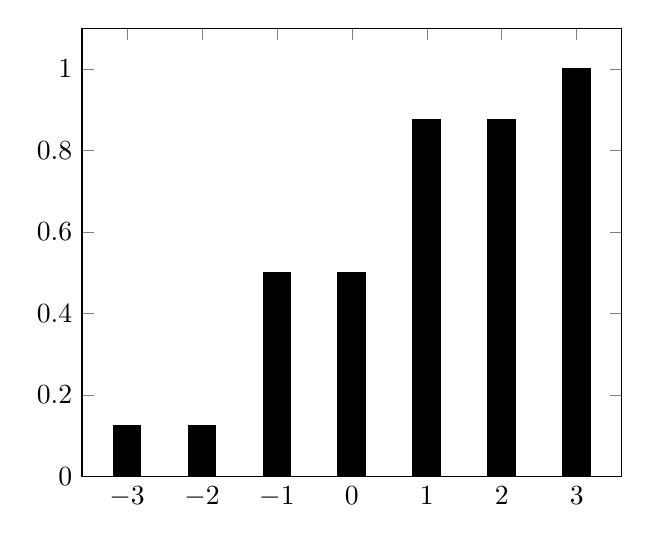
\begin{tikzpicture}
        \begin{axis}[
            ymin=0
        ]
        \addplot[ybar, fill=black] coordinates {
            (-3,0.125)
            (-2,0.125)
            (-1,0.5)
            (0,0.5)
            (1,0.875)
            (2,0.875)
            (3,1)
        };
        \end{axis}
        \end{tikzpicture}
        \caption{CDF}
        \label{fig:cdf2}
    \end{subfigure}
    \end{figure}
\end{parts}

\miquestion
\begin{parts}
    \part In any given roll, the outcome can only be greater than or equal to one. Therefore,
    $$P(X\geq1)=1$$
    \part In order for the minimum to be 2 or more, not a single dice can roll a 1. Hence, for each dice we are only left with 5 outcomes out of 6,
    $$P(X\geq2)=\frac{5}{6}\cdot\frac{5}{6}\cdot\frac{5}{6}\cdot\frac{5}{6}=\left(\frac{5}{6}\right)^4=0.4822530864$$
    \part $P(X\leq k)$ for all values of $k$,
    $$P(X\leq1)=1-P(X\geq2)=1-\left(\frac{5}{6}\right)^4=0.5177469136$$
    $$P(X\leq2)=1-\left(\frac{4}{6}\right)^4=0.8024691358$$
    $$P(X\leq3)=1-\left(\frac{3}{6}\right)^4=0.9375$$
    $$P(X\leq4)=1-\left(\frac{2}{6}\right)^4=0.987654321$$
    $$P(X\leq5)=1-\left(\frac{1}{6}\right)^4=0.9992283951$$
    $$P(X\leq6)=1$$
    \begin{figure}[h]
        \centering
        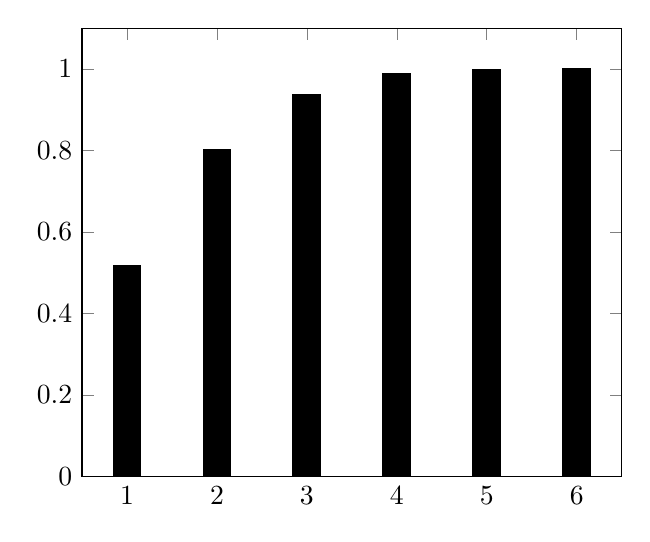
\begin{tikzpicture}
        \begin{axis}[
            ymin=0
        ]
        \addplot[ybar, fill=black] coordinates {
            (1,0.5177469136)
            (2,0.8024691358)
            (3,0.9375)
            (4,0.987654321)
            (5,0.9992283951)
            (6,1)
        };
        \end{axis}
        \end{tikzpicture}
        \caption{CDF}
        \label{fig:cdf3}
    \end{figure}
\end{parts}

\end{questions}

\end{document}
